\documentclass[10pt,center]{beamer}

%%%%%%%%%%% Lo que viene  a continuacion es el tipo de presentacion que quieres, 
% las presentaciones se llaman con nombres de ciudades puedes cambiarlas y tomar
%%%%%%%%la que mas te guste.
\mode<presentation> {
  %\usetheme{Frankfurt}
  %\usetheme{Warsaw}
  %\usetheme{Darmstadt}
  %\usetheme{Dresden}
  \usetheme{Singapore}
  %\usetheme{Bergen}
  %\usetheme{Boadilla}
  %\usetheme{BerKeley}
  \setbeamercovered{transparent}
  \setbeamertemplate{footline}[frame number]
  %\setbeamertemplate{background canvas}[vertical shading][bottom=red!20,top=yellow!30]
  \setbeamertemplate{headline}{}
  %\setbeamerfont{caption}{size=\tiny}
%%%%%%%%%%%%%%%%%%%%%%%%%%%%%%%%%%
%%%%%%% aqui vienen los colores

  %\usecolortheme{crane}
  %\usecolortheme{seahorse}
  \usecolortheme{whale}
  %\usecolortheme{rose}
  %\usecolortheme{orchid}
} \usepackage{alltt}



%%%%%%%los paquetes. 
\usepackage{amssymb,amsmath,latexsym}
%\usepackage[mathcal]{euscript}
%\usepackage[polish]{babel}
%\usepackage{dsfont}
%\usepackage[normalem]{ulem}
\usepackage{enumerate}
%\usepackage[all,2cell,dvips]{xy} \UseAllTwocells \SilentMatrices

\usepackage{verbatim}
\usepackage{float}

\usepackage[utf8]{inputenc}
\usepackage{url}
\usepackage{makeidx}
\usepackage[procnames]{listings}
\usepackage{color}
\usepackage{graphicx} % graficos
\usepackage{subfig}
\usepackage{tabularx}
%\usepackage{subcaption}
\captionsetup{compatibility=false}
\usepackage[export]{adjustbox}
\usepackage[spanish]{babel}
\usepackage{mathtools}
\usepackage{svg}
\usepackage{caption}

\title{Transferencia de Estilo en Fotografias mediante Redes Neuronales Convolucionales}
%
%
\author{Ariel Wolfmann}

%
\institute{Facultad de Matemática, Astronomía, Física y Computación\\
	  Universidad Nacional de Córdoba}

\date{28 de Julio, 2017}


\begin{document}
%%%%%%%%%%%%%%%%%%%%%%%%%%%PAGINA DEL TITULO
\begin{frame}
  \titlepage
\end{frame}

%%%%%%%%%%%%%%%%%  tODO LO QUE QUIERAS PONER EN LOS FRAMES.
\begin{frame}
  \frametitle{Agenda}
  \tableofcontents
\end{frame}

\section{Introducción}
\begin{frame}
  \frametitle{Introducción}
  \framesubtitle{Contexto}
  Aplicaciones de efectos en fotografias:
    \begin{figure}[H]
      \begin{center}
	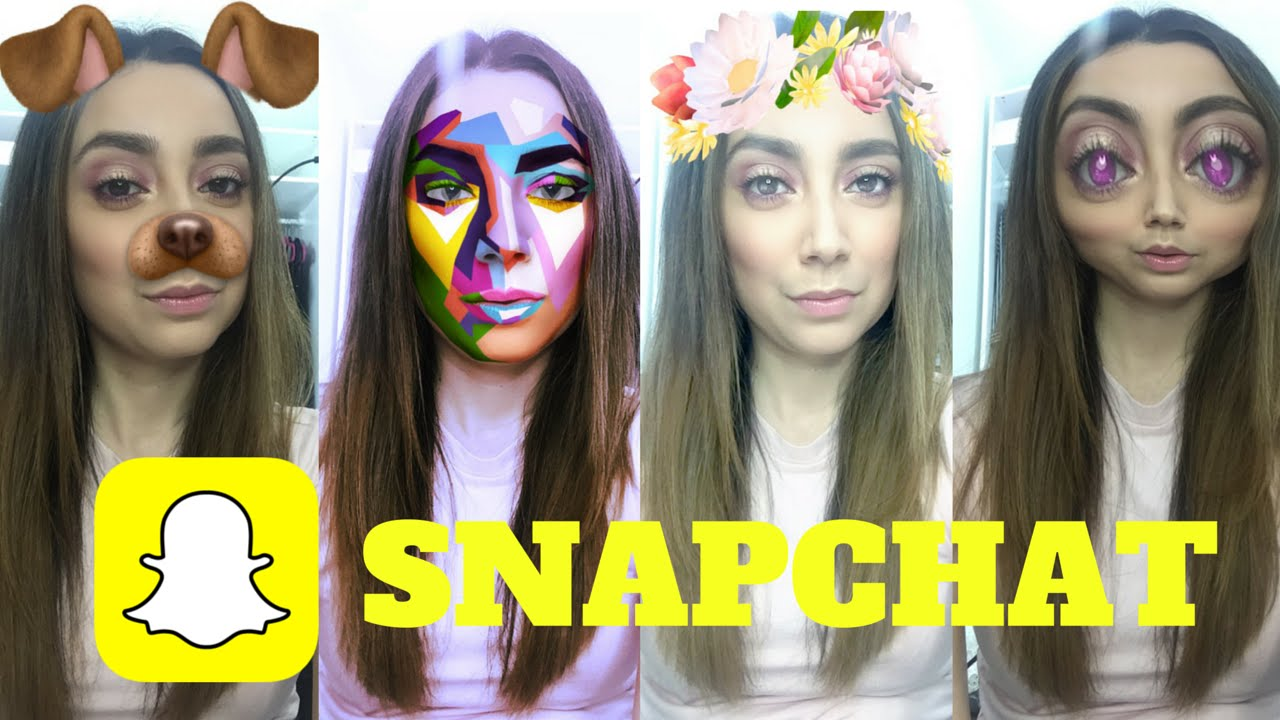
\includegraphics[width=0.8\linewidth]{./img/filtro_snapchat.jpg}
      \end{center}
    \end{figure}
\end{frame}	

\begin{frame}
  \frametitle{¿Como se representa una imágen?}
  Arreglo de píxeles ordenados, puede tener 1 o más canales
    \begin{figure}[H]
      \begin{center}
	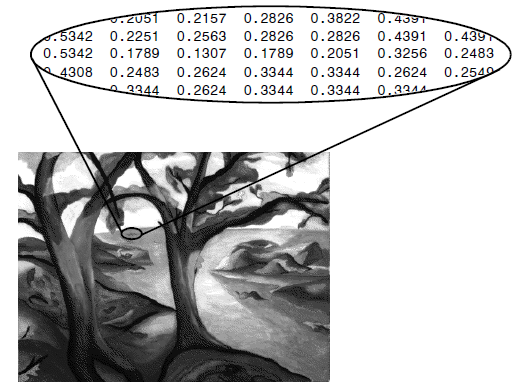
\includegraphics[width=0.8\linewidth]{./img/image_pixel.png}
      \end{center}
    \end{figure}
\end{frame}
  
\begin{frame}
  \frametitle{Aprendizaje automático en visión por computadoras}
  \begin{itemize}
    \item \textbf{Visión por computadoras} (Computer Vision): Comprensión de alto nivel sobre imágenes digitales, busca automatizar tareas del sistema visual humano.
    \item \textbf{Aprendizaje automático} (Machine Learning): Algortimos que otorgan a las computadoras la habilidad de aprender y hacer predicciones sobre los datos de entrada. 
  \end{itemize}
  
  \begin{figure}[H]
    \begin{center}
      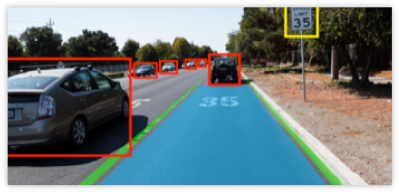
\includegraphics[height=0.4\textheight]{./img/nvidia_car_detection.png}
    \end{center}
    \caption{Vehiculos autónomos}
  \end{figure}    
\end{frame}
  
\begin{frame}
  \frametitle{Transferencia de estilo}
  A partir de una imagen de contenido y una imagen de estilo se genera una nueva imagen que combina ambas.
  \begin{figure}[h]
    \begin{center}
      \subfloat[\small Estilo]{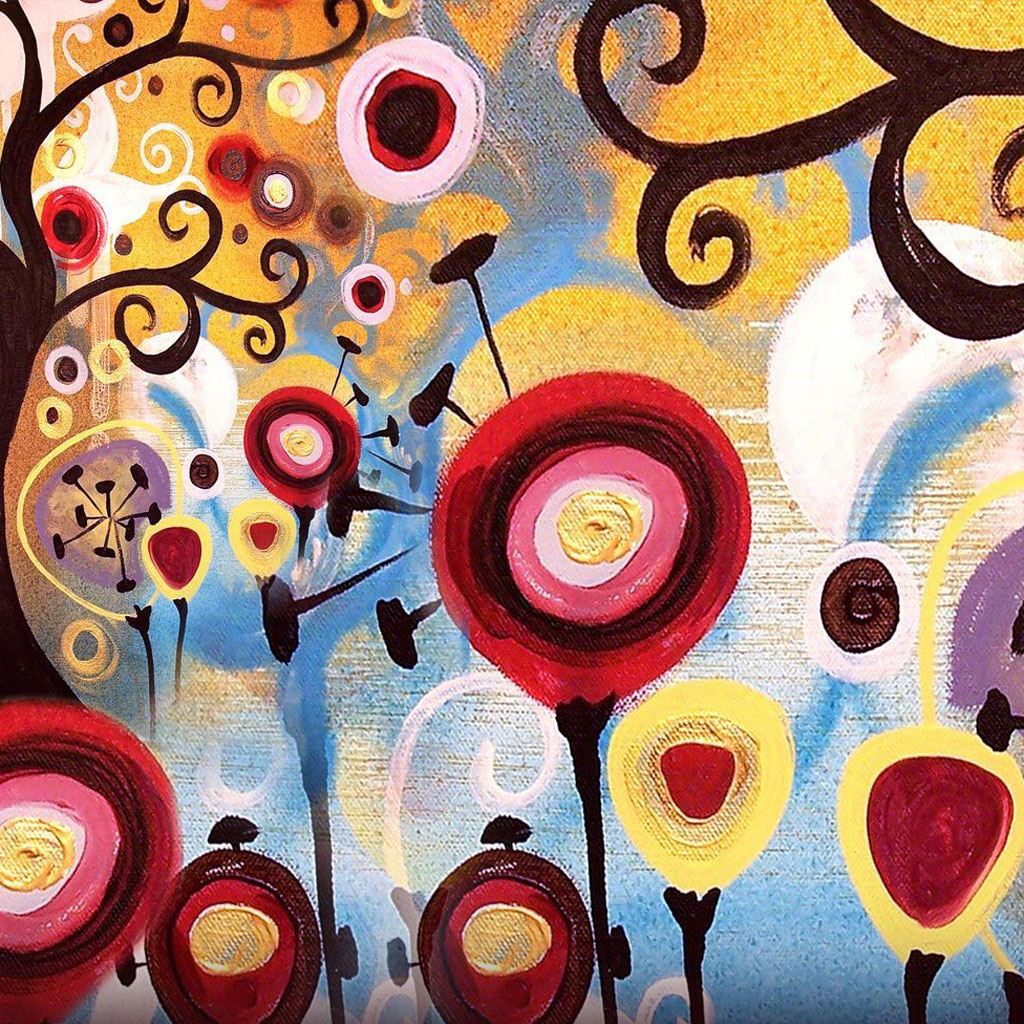
\includegraphics[height=0.25\textheight]{./img/jhonson_style_candy.jpg}} \hspace{1.0cm}
      \subfloat[\small Contenido]{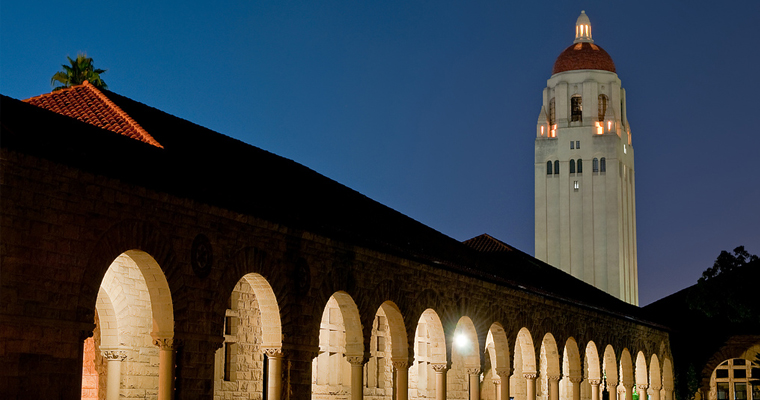
\includegraphics[height=0.25\textheight]{./img/jhonson_content_tower.jpg}} \hspace{1.0cm}
      \subfloat[\small Resultado]{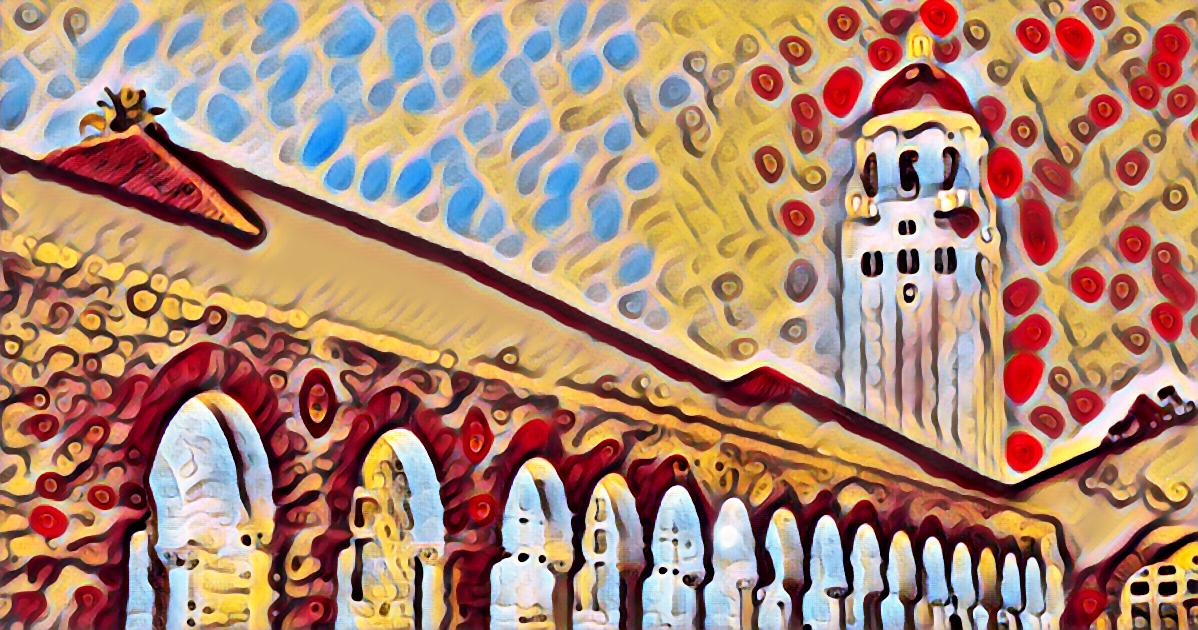
\includegraphics[height=0.25\textheight]{./img/jhonson_result_tower_candy.jpg}}
      
    \end{center}
  \end{figure}  
\end{frame}	
  
  
\section{Aprendizaje Automático}

\begin{frame}
   \frametitle{Aprendizaje Automático}
  
  \begin{itemize}
    \item Se encuentra en la intersección de las cs. de la computación y el aprendizaje estadístico
    \item Aprendizaje supervisado vs no supervisado: etiquetas 
  \end{itemize}
%  
  \begin{figure}[h]
    \begin{center}
      \subfloat[Clasificación lineal]{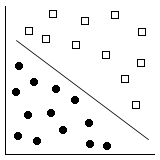
\includegraphics[ height=0.35\textheight]{./img/linear_svm.png}}
      \subfloat[Clustering]{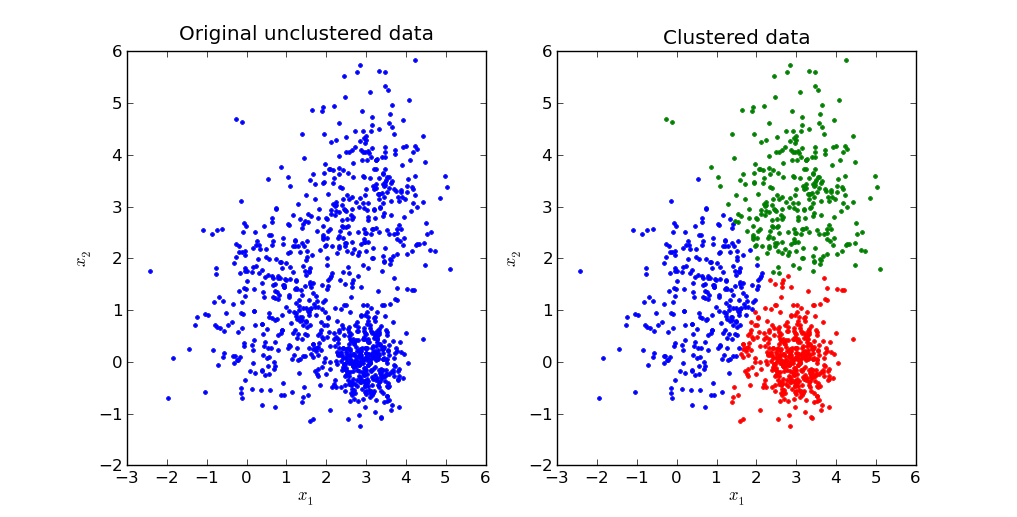
\includegraphics[height=0.40\textheight]{./img/stackoverflow_clustering.png}}
    \end{center}
  \end{figure}  
%  
\end{frame}

\begin{frame}
  \frametitle{Clasificación de imágenes}
  \begin{itemize}
    \item Representación de la información: \textit{features}
    \item Enfoque clásico vs enfoque aprendizaje profundo
    \begin{itemize}
      \item Enfoque clásico: \textit{features} predefinidas para entrenar el modelo.
      \item Enfoque aprendizaje profundo: Tanto las \textit{features} como el modelo se entrenan y aprenden en conjunto.
    \end{itemize}
  \end{itemize}
  \begin{figure}[h]
    \begin{center}
	    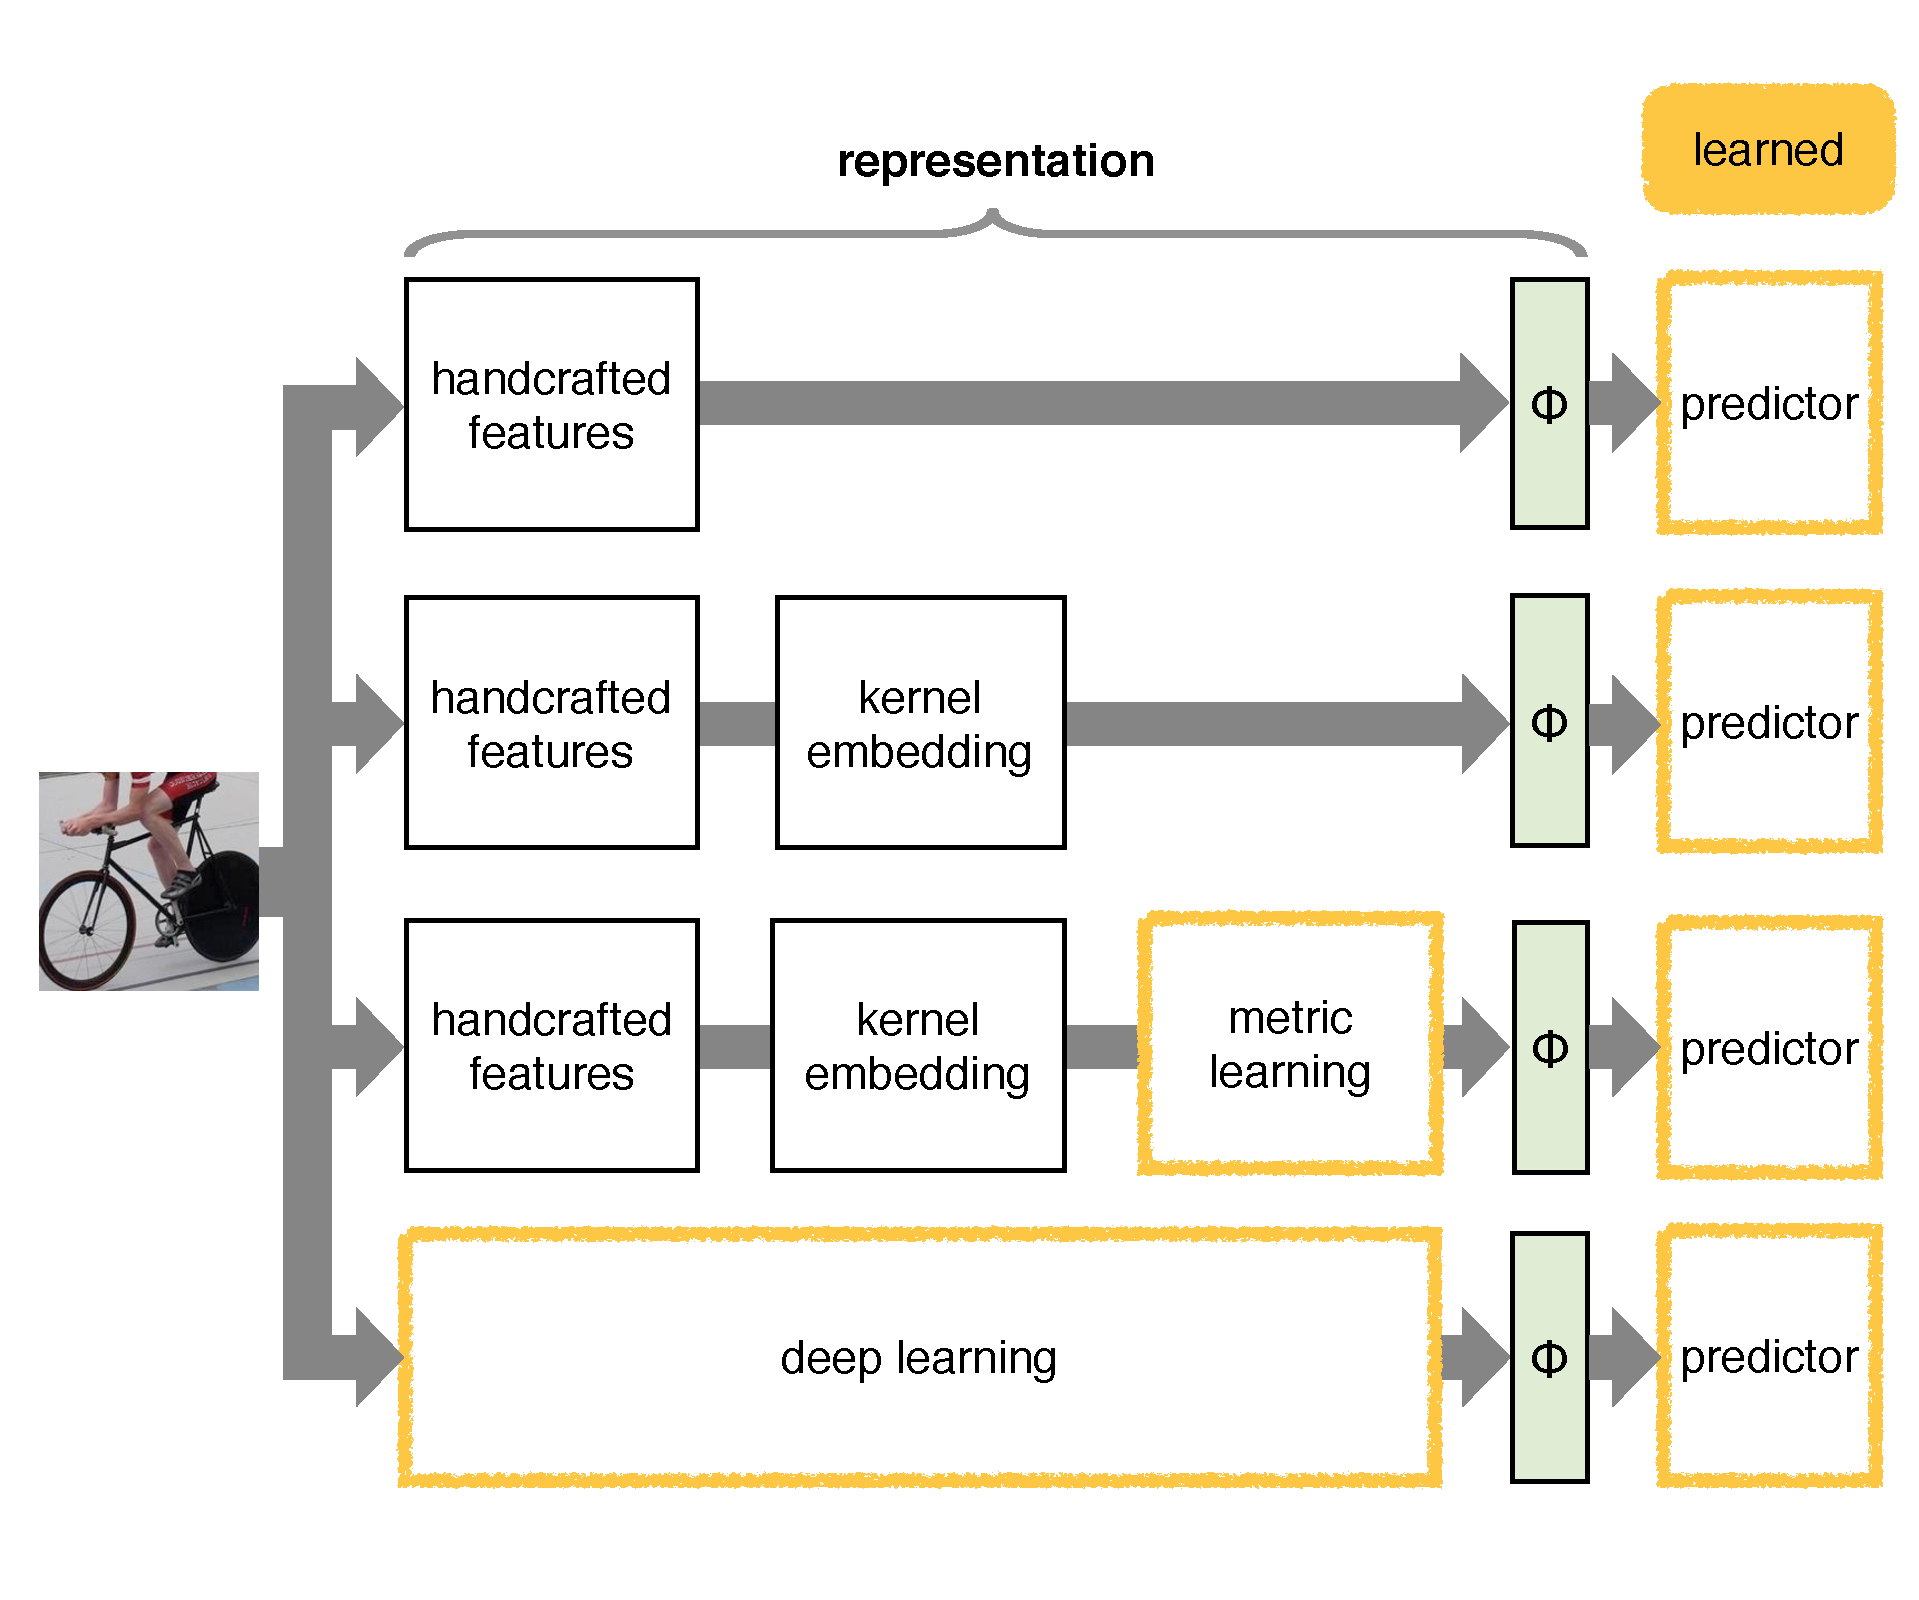
\includegraphics[height=0.6\textheight]{./img/vedaldi_shallow_deep.pdf}
    \end{center}
  \end{figure}
\end{frame}

\begin{frame}
  \frametitle{¿En que consiste el aprendizaje?}
  \begin{itemize}
    \item Funcion de predicción: mapeo $f_{\overrightarrow{w}}: \mathcal{X} {\rightarrow} \{1,\dots,K\}$
    \item Objetivo del aprendizaje: ajustar $\overrightarrow{w}$ para mejorar la predicción.
    \item Optimización: minimizar función de pérdida (diferencia entre la predicción y el valor esperado).
  \end{itemize}
\end{frame}

\begin{frame}
  \frametitle{Descenso por el gradiente}
    Optimizar mediante refinamiento iterativo, siguiendo la dirección del gradiente de la función de pérdida ($L(.)$).
  \begin{equation*}
    w_{n+1} = w_n - \nabla L(w_n)
  \end{equation*}
  \begin{figure}[h]
    \begin{center}
	    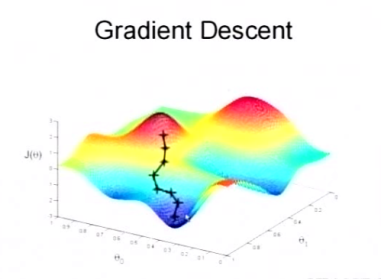
\includegraphics[height=0.4\textheight]{./img/gradient_descent_1.png}
    \end{center}
  \end{figure}
\end{frame}

\section{Redes Neuronales Artificiales}
\begin{frame}
  \frametitle{Redes Neuronales Artificiales}
    \begin{itemize}
      \item Versión compleja de un clasificador lineal, utilizando funciones no lineales.
      \item Conjunto de unidades de cómputo (neuronas) conectadas en un grafo acíclico organizadas por capas. 
      \item Las unidades de una capa solo se conectan con neuronas de sus capas adyacentes.
    \end{itemize}

    \begin{figure}[ht]
      \begin{center}
	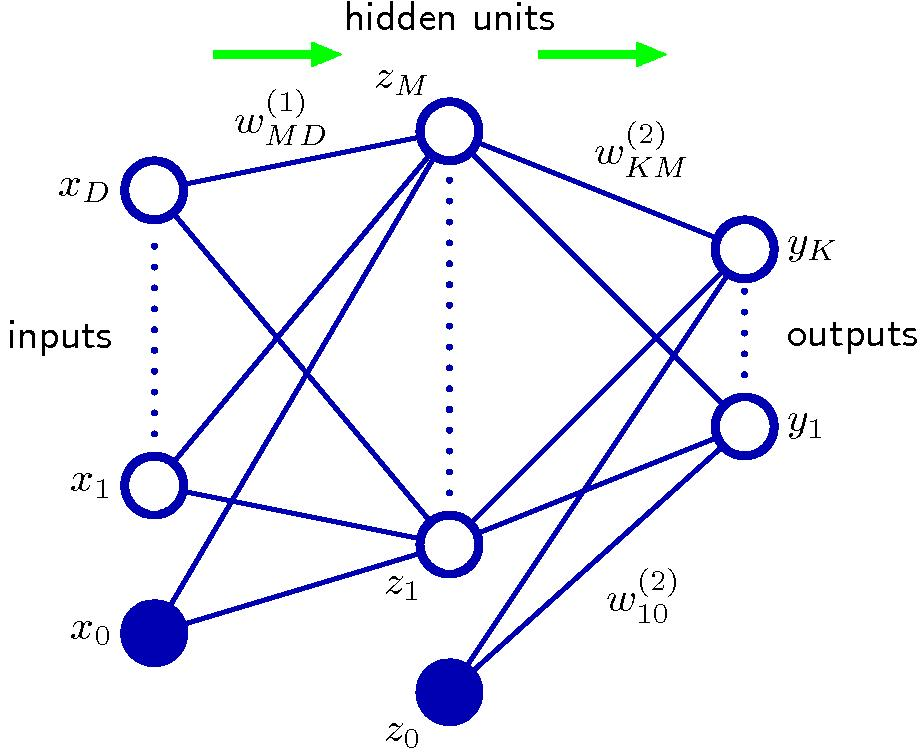
\includegraphics[height=0.5\textheight]{./img/bishop_neural_network.jpg}
      \end{center}
      \caption{Red Neuronal Artificial}
    \end{figure}
\end{frame}

\begin{frame}
    \frametitle{Entrenando una red neuronal}
    Ciclos de 2 pasos
    \begin{enumerate}
      \item Paso hacia adelante: evaluación de la red en base al dato de entrada.
      \item Retropropagación: corrección de los pesos internos de la red, según el gradiente de la función de pérdida.
    \end{enumerate}

    \begin{figure}[ht]
      \begin{center}
      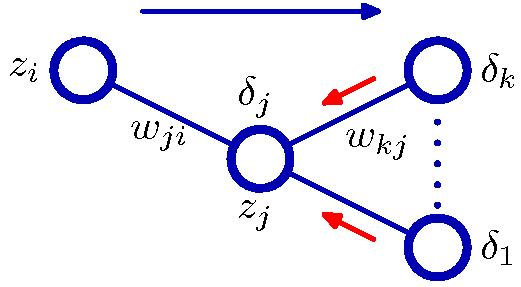
\includegraphics[width=0.5\linewidth]{./img/bishop_backpropagation.jpg}
      \end{center}
    \end{figure}
\end{frame}


\section{Redes Neuronales Convolucionales}
\begin{frame}
  \frametitle{Redes Neuronales Convolucionales - CNN}
    \begin{itemize}
      \item Redes neuronales que asumen que sus entradas son \textbf{imágenes}.
      \item Codifican propiedades de la imagen en la arquitectura de la red mediante:
      \begin{itemize}
	\item \textbf{Volumen}: Las capas y los resultados intermedios (\textit{feature maps}) se ordenan en 3 dimensiones.
	\item \textbf{Localidad espacial}: píxeles cercanos suelen estar correlacionados.
	\item \textbf{Submuestreo}: reduce el tamaño de la salida tomando un valor que representa a su región. 
	Otorga tolerancia a desplazamientos y variaciones.
	\item \textbf{Convolución}:
	  \begin{itemize}
	    \item Se aplica un filtro (matriz de 3x3 o 5x5) desplazándolo por toda la imagen.
	    \item Se obtiene una nueva imagen resultante de aplicar el filtro.
	    \item Permite detectar \textit{features}. 
	  \end{itemize}
      \end{itemize}
    \end{itemize}
    \begin{figure}[h]
    \captionsetup[subfigure]{labelformat=empty}
      \begin{center}
      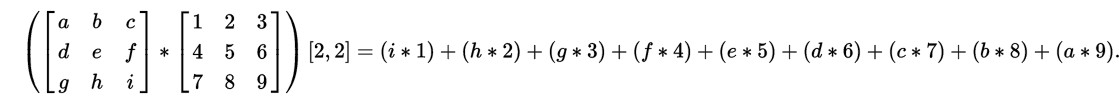
\includegraphics[width=\textwidth]{./img/convolution_wiki.jpg}
      \end{center}
    \end{figure}
\end{frame}
  
\begin{frame}
  \frametitle{Estructura de la CNN}
    \begin{itemize}
     \item \textbf{Capa de Entrada}: píxeles en bruto.
     \item \textbf{Capa de Convolución}
     \begin{itemize}
      \item Produce un \textit{feature map} por cada filtro (aumenta la profundidad del volumen).
      \item Luego de la convolución se aplica una función no lineal (por ej. $f(x) = max(0,x)$)
     \end{itemize}
     \item \textbf{Capa de Submuestreo}: reduce dimensiones espaciales (largo y ancho).
     \item \textbf{Capa de Salida}: realiza predicción final. 
    \end{itemize}
  \begin{figure}[h]
  \captionsetup[subfigure]{labelformat=empty}
    \begin{center}
    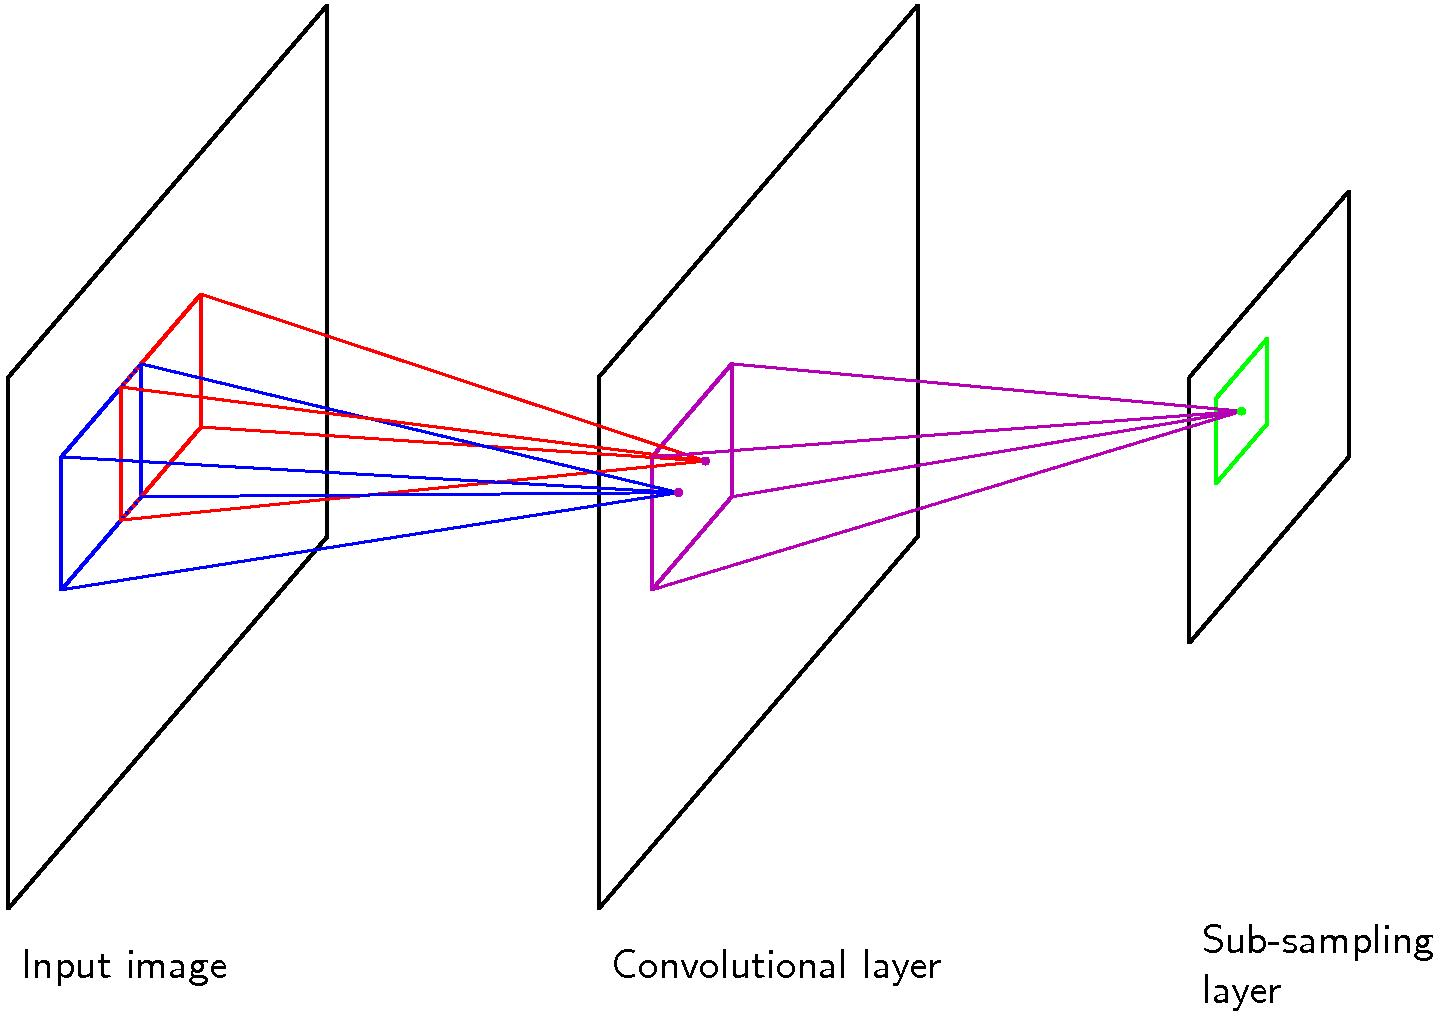
\includegraphics[height=0.45\textheight]{./img/bishop_cnn.jpg}
    \end{center}
  \end{figure}
\end{frame}

\section{Ajuste Fino}
\begin{frame}
  \frametitle{Ajuste Fino - Finetuning}
  Adaptar una red pre-entrenada a un problema similar.
    \begin{itemize}
     \item Toma una red pre-entrenada y un pequeño conjunto de datos.
     \item Reemplaza la última capa de la red por una adaptada al problema.
     \item Reentrena la red comenzando con los pesos predefinidos, ajustándolos a los nuevos datos.
    \end{itemize}
  \begin{figure}[h]
  \captionsetup[subfigure]{labelformat=empty}
    \begin{center}
      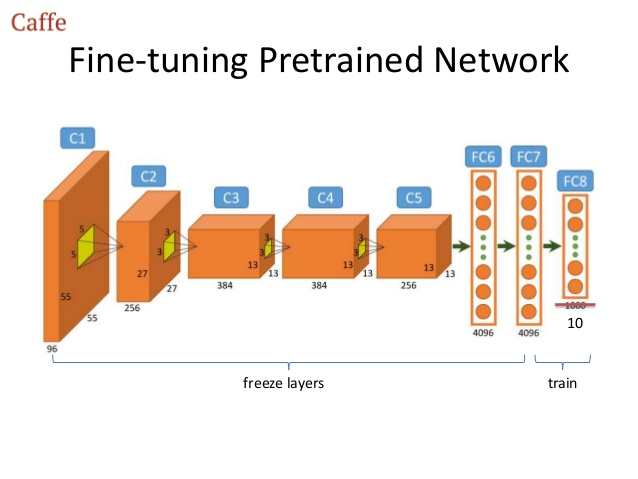
\includegraphics[height=0.6\textheight]{./img/fine_tuning.jpg}
    \end{center}
  \end{figure}
\end{frame}


\section{Algoritmo de transferencia de estilo}
\begin{frame}
 \frametitle{Algoritmo de transferencia de estilo}
 \begin{itemize}
    \item Algoritmo publicado por Gatys et. al.
    \item Toma como entrada 2 imágenes: una de contenido y otra de estilo.
    \item Genera iterativamente una imagen artificial, compuesta por el contenido de una imagen y el estilo de la otra.
    \item Utiliza los mapas de características de CNN para calcular el estilo y el contenido.
 \end{itemize}
    \begin{figure}[h]
    \captionsetup[subfigure]{labelformat=empty}
    \begin{center}
     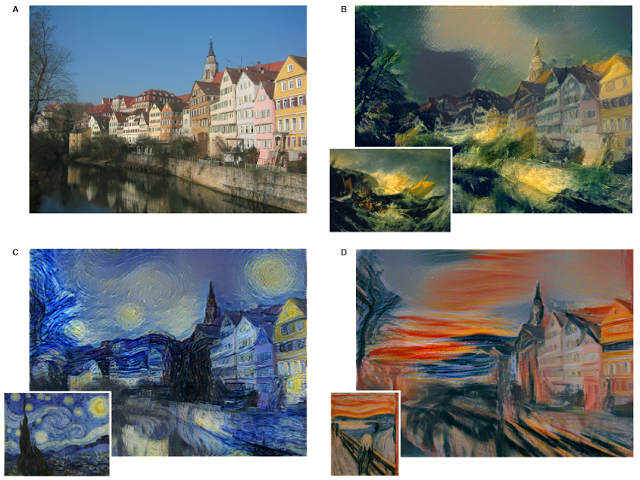
\includegraphics[width=0.5\textwidth]{./img/gatys_style_transfer.png}
    \end{center}
  \end{figure} 
\end{frame}

\begin{frame}
  \frametitle{Reconstrucciones del estilo y contenido utilizando una CNN}
   \begin{figure}[h]
   \captionsetup[subfigure]{labelformat=empty}
    \begin{center}
     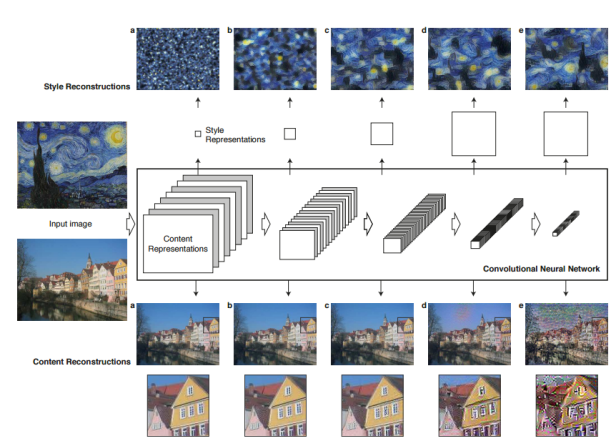
\includegraphics[width=\textwidth]{./img/gatys_1.png}
    \end{center}
  \end{figure} 
\end{frame}


\begin{frame}
 \frametitle{Contenido}
  \begin{itemize}
   \item \textbf{Representación del contenido}: \textit{feature map} de una de las últimas capas de la red.
   \item \textbf{Mapa de características de la imagen de contenido}: matriz $F^l$, donde $F_{i,j}^l$ es la respuesta del $i$-esimo filtro en la posición $j$ de la capa $l$.
   \item \textbf{Función de pérdida del contenido}: Error cuadrático medio entre los \textit{feature maps} de la imagen generada $F$ y la imagen de contenido $P$.
  \end{itemize}
  \begin{equation*}
    L_{contenido}(\overrightarrow{p},\overrightarrow{x}, l) = \frac{1}{2} \sum_{i,j} (F_{i,j}^l - P_{i,j}^l)^2
  \end{equation*}
\end{frame}

\begin{frame}
 \frametitle{Estilo}
  \begin{itemize}
    \item \textbf{Representación del estilo}: correlación entre los valores del \textit{feature map}.
    \item \textbf{Correlación de características}: matriz de Gramm $G^l \in R^{N_l \times N_l}$, en la cual $G_{i,j}^l$ se calcula como el producto punto entre los vectores
      de los \textit{feature maps} $i$ y $j$ en la capa $l$:
	\begin{equation*}
	  G_{i,j}^l = \sum_{k} F_{i,k}^l F_{j,k}^l
	\end{equation*}
  \end{itemize}

\end{frame}

\begin{frame}
  \frametitle{Función de pérdida de estilo}
  \begin{itemize}
   \item Suma pesada de los errores entre el estilo calculado de la imagen generada y la imagen de estilo, de varias capas.
   \item La función de pérdida de estilo de cada capa es:
      \begin{equation*}
	E_l = \sum_{i,j} (G_{i,j}^l - A_{i,j}^l)^2
      \end{equation*}
   \item La función de pérdida de estilo total: combinación lineal de las funciones de pérdida de estilo de cada capa:
      \begin{equation*}
	L_{estilo}(\overrightarrow{a},\overrightarrow{x}) = \sum_{l=0}^{L} w_l E_l
      \end{equation*}
  \end{itemize}
\end{frame}

\begin{frame}
  \frametitle{Transferencia de estilo}
  \begin{figure}[h]
    \begin{center}
      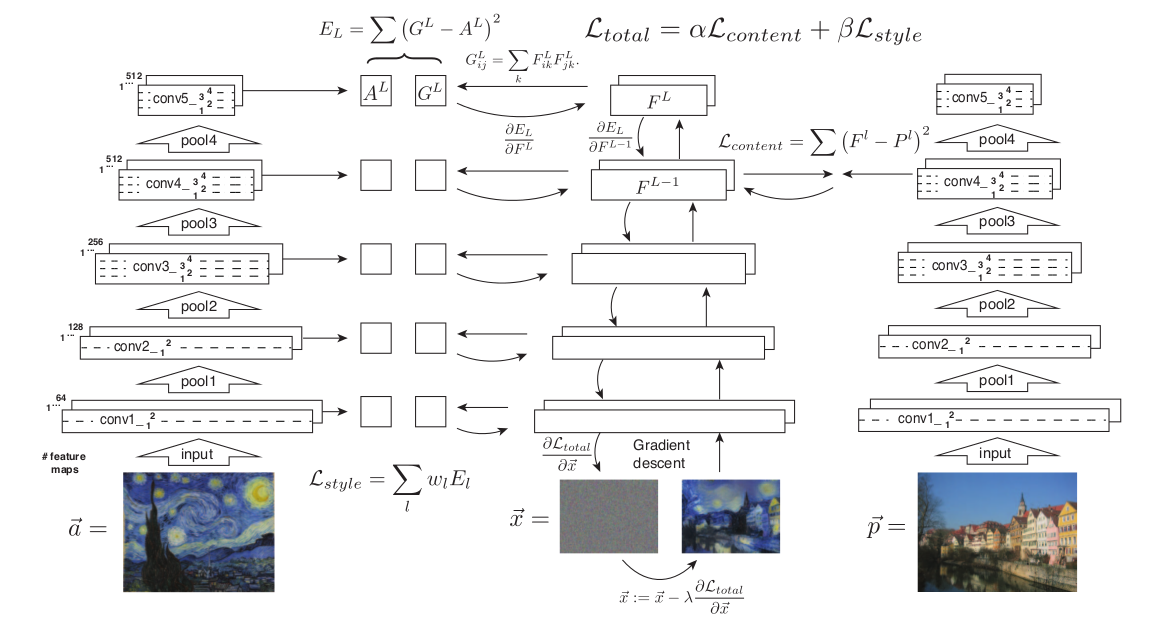
\includegraphics[width=\textwidth]{./img/gatys_method.png}
    \end{center}
  \end{figure}
\end{frame}

\begin{frame}
  \frametitle{Hiperparámetros}
  \begin{itemize}
   \item Número de iteraciones: Determina cuantas veces se ejecuta el método de descenso por el gradiente para minimizar la función de pérdida. \vspace{0.5cm}
   \item Red Convolucional: Dependiendo de la red convolucional que se utilice, cambia el tamaño de los mapas de características, las capas, etc. \vspace{0.5cm}
   \item Capas de la red para la representación de estilo y sus respectivos pesos ($w_l, l \in \{1 \dots L\}$). \vspace{0.5cm}
   \item Capa de la red para la representación del contenido. \vspace{0.5cm}
   \item Factores de peso para las funciones de pérdida de estilo y contenido en la función de pérdida total $(\alpha, \beta)$. \vspace{0.5cm}
   \item otros..
  \end{itemize}
\end{frame}

\section{Elección automática de hiperparámetros}
\begin{frame}
  \frametitle{Problema: elección automática de hiperparámetros}
  \begin{itemize}
   \item El número de iteraciones se detectó como el principal factor de influencia en el resultado del algoritmo. \vspace{0.5cm}
   \item En el arte, las evaluaciones suelen ser cualitativas.
   \begin{itemize}
    \item Es necesario definir un criterio cuantitativo de evaluación para poder determinar si un resultado es aceptado o no. \vspace{0.5cm}
   \end{itemize}
  \item Objetivo: generar una imagen aceptada en la menor cantidad de iteraciones posible.
  \end{itemize}

\end{frame}

\begin{frame}
 \frametitle{Solución propuesta}
  \begin{itemize}
   \item \textbf{Módulo de generación de imágen}: transferencia de estilo.
   \item \textbf{Módulo de evaluación}: reconocimiento de estilo.
   \item \textbf{Definir critero de aceptación cuantitativo}: estilo cercano a la imagen objetivo .
  \end{itemize}
  \begin{figure}[h]
  \captionsetup[subfigure]{labelformat=empty}
    \begin{center}
      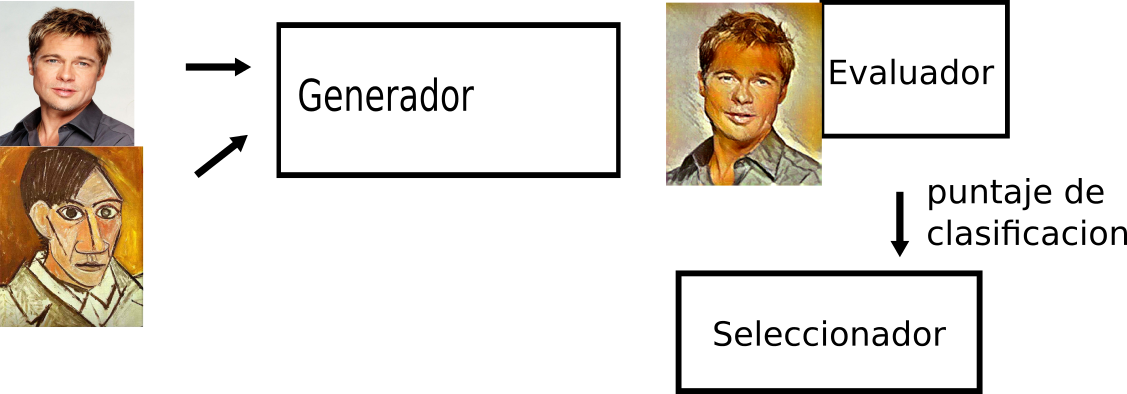
\includegraphics[width=\linewidth]{./img/diagrama.png}
    \end{center}
    \caption{Diagrama de interacción entre los distintos módulos propuestos}
  \end{figure}
\end{frame}

\section{Experimentos}
\begin{frame}
  \frametitle{Reconocimiento de estilo}
  \begin{itemize}
    \item Finetuning sobre red preentrenada para clasificar objetos. \vspace{0.5cm}
    \item Datos provenientes de WikiArt. \vspace{0.5cm}
    \item POC sobre los 10 principales estilos. \vspace{0.5cm}
  \end{itemize}
\end{frame}

\begin{frame}
  \frametitle{Estilos}
  \captionsetup{font=scriptsize}
  \begin{figure}
  \captionsetup[subfigure]{labelformat=empty}
      \begin{center}
      %\def\tabularxcolumn##1{m{##1}}
      \begin{tabularx}{\textwidth}{@{}cXX@{}}
      %
      \begin{tabular}{ccccc}
	\subfloat[\small Modernismo]{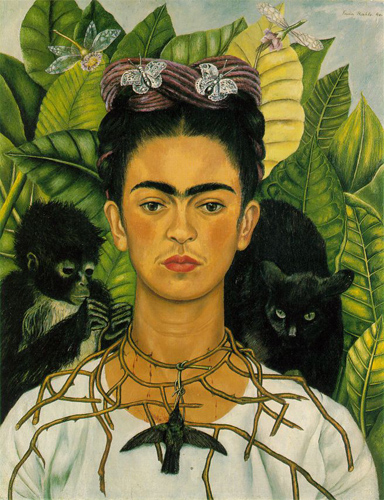
\includegraphics[height=0.15\textheight]{./img/frida_kahlo.jpg}}
	& \subfloat[\small Impresionismo]{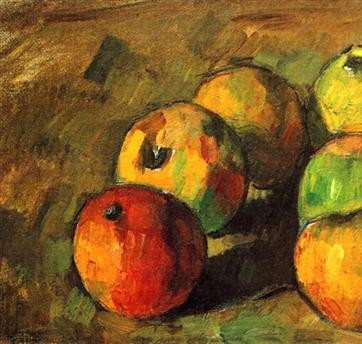
\includegraphics[height=0.15\textheight]{./img/cezanne.jpg}}
	& \subfloat[\small Surrealismo]{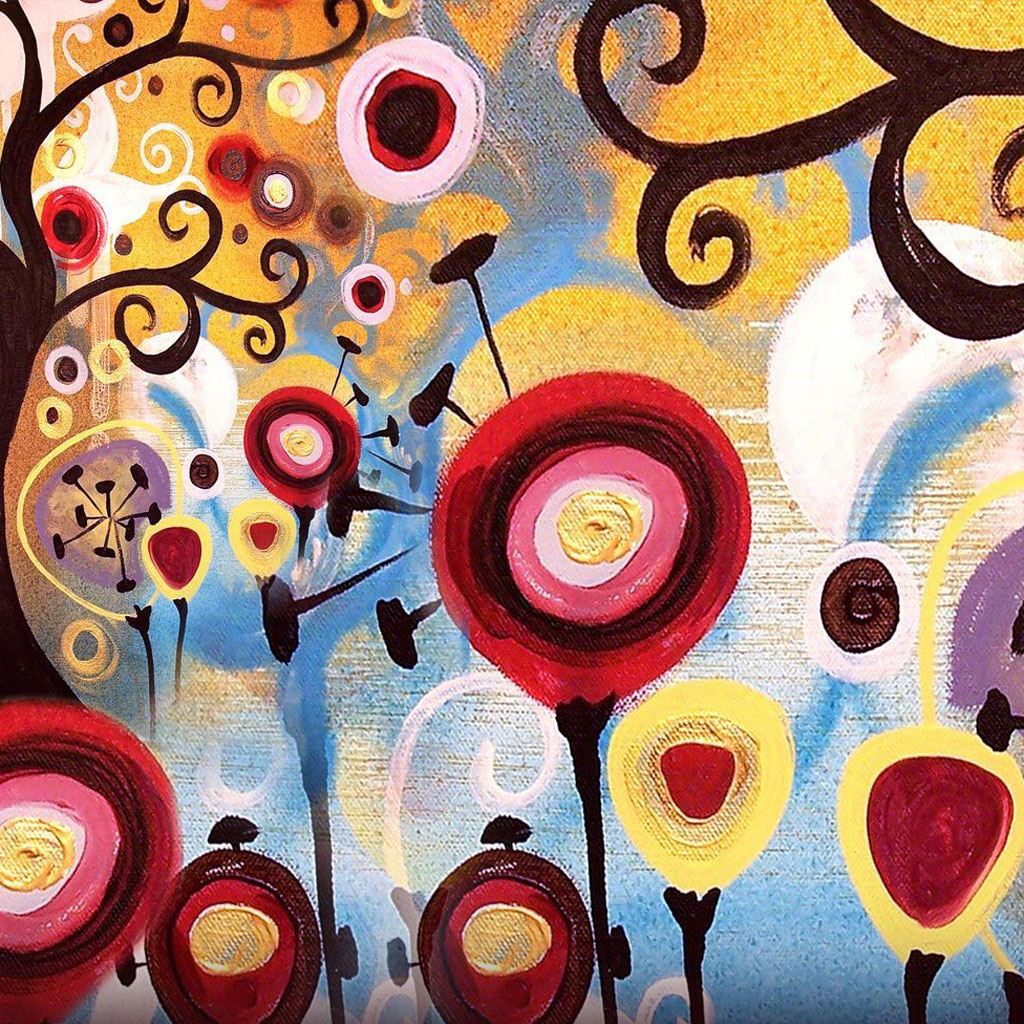
\includegraphics[ height=0.15\textheight]{./img/jhonson_style_candy.jpg}}
	& \subfloat[\small Post Impresionismo]{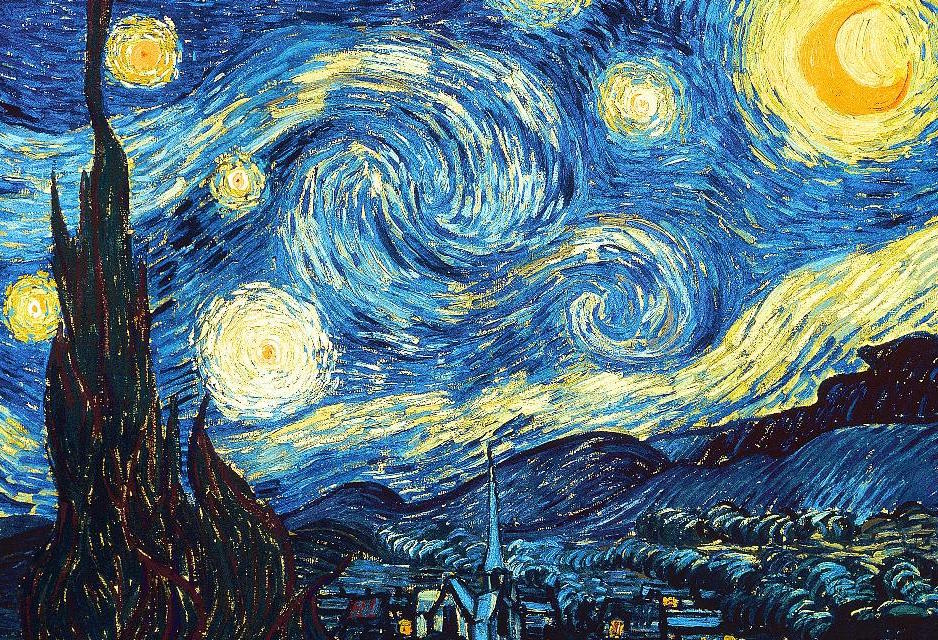
\includegraphics[height=0.15\textheight]{./img/starry_night.jpg}}
	& \subfloat[\small Simbolismo]{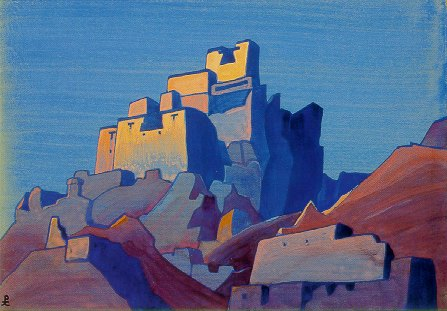
\includegraphics[ height=0.15\textheight]{./img/nicholas-roerich_chiktan-citadel-in-himalayas.jpg}}\\
	\subfloat[\small Neo Clasisimo]{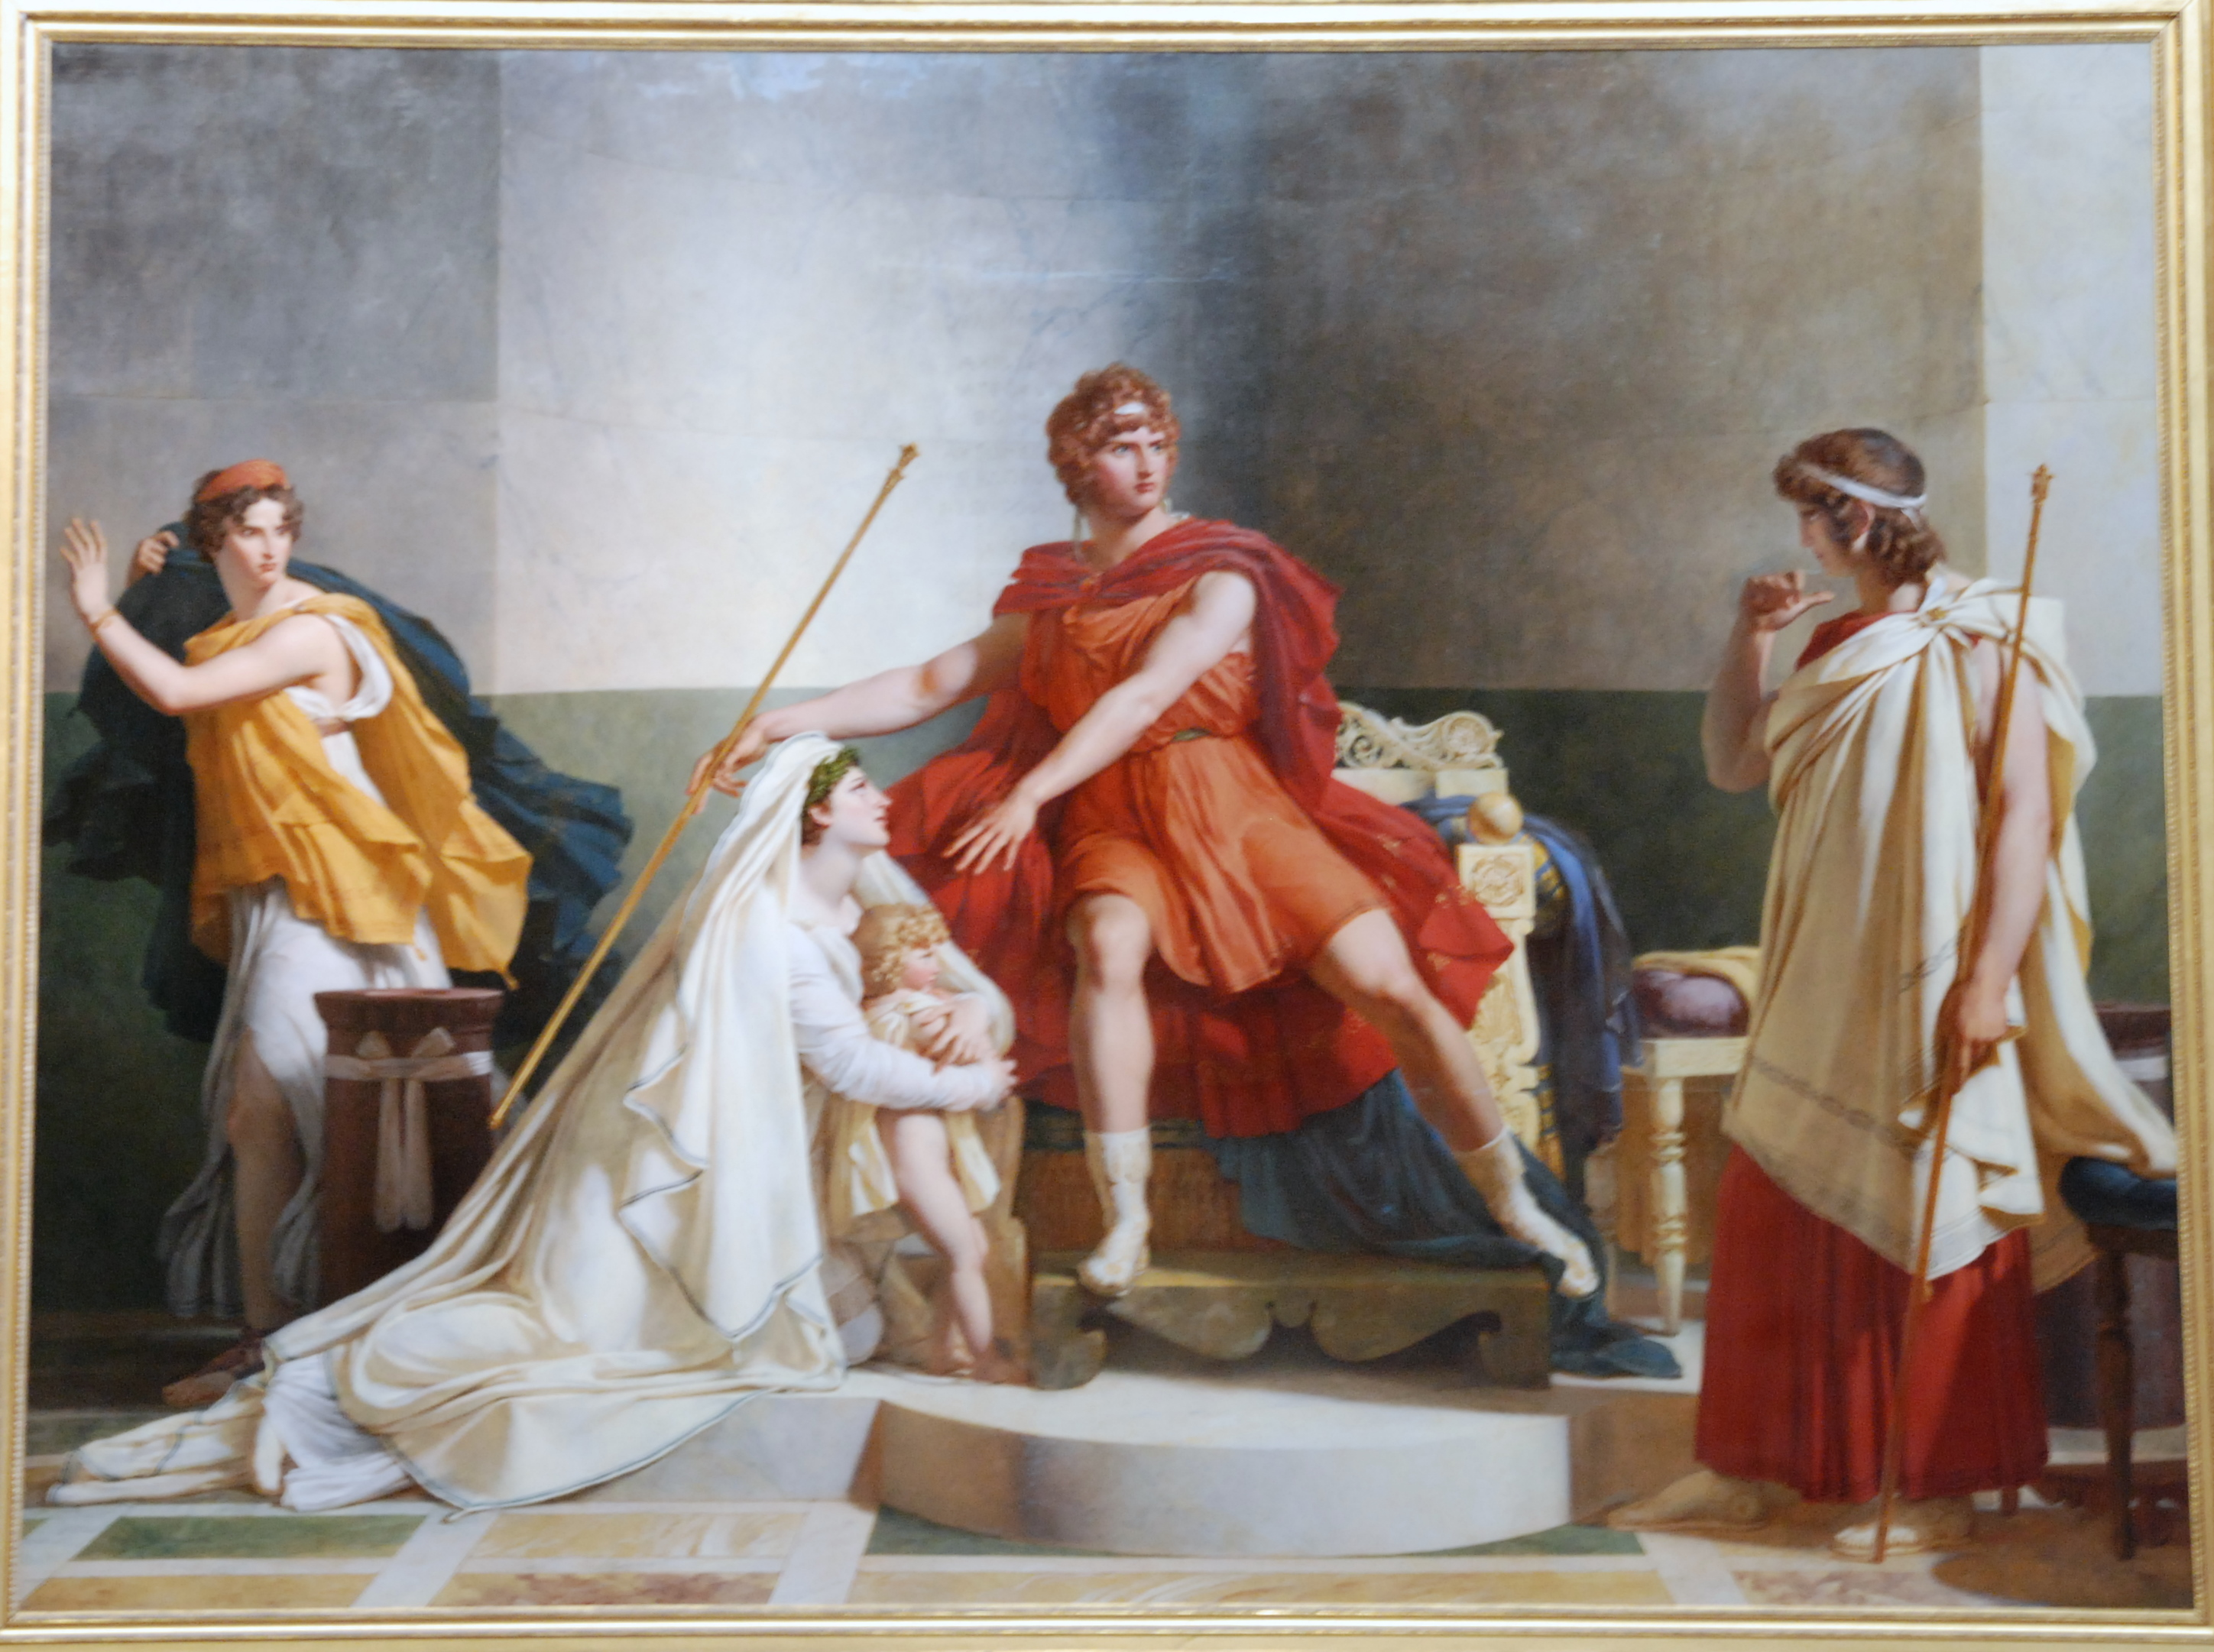
\includegraphics[height=0.15\textheight]{./img/pierre-narcisse-guerin_not-detected.jpg}}
	& \subfloat[\small Romanticismo]{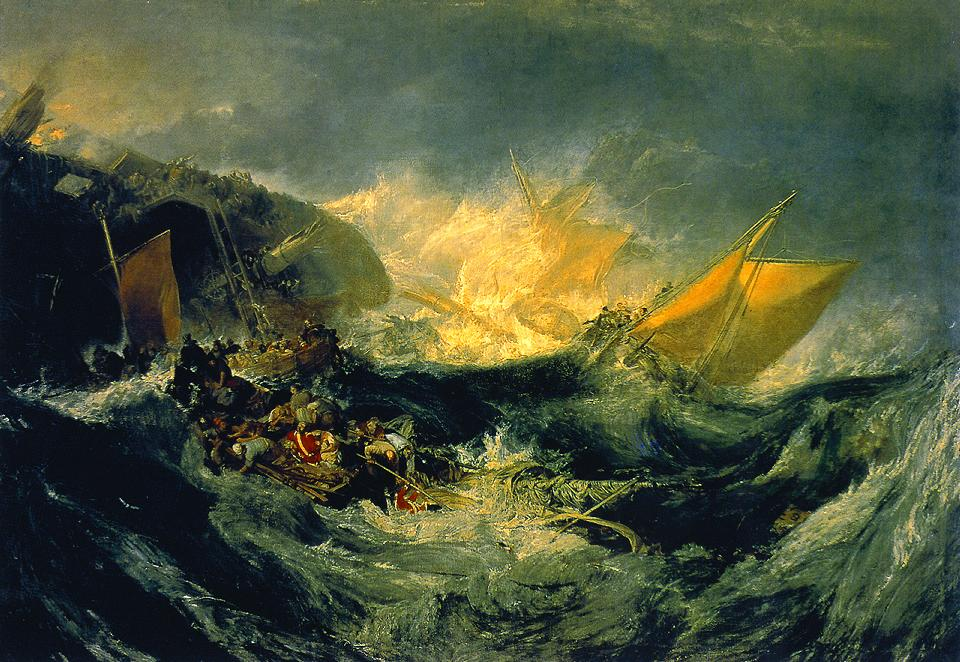
\includegraphics[height=0.15\textheight]{./img/shipwreck.jpg}}
	& \subfloat[\small Barroco]{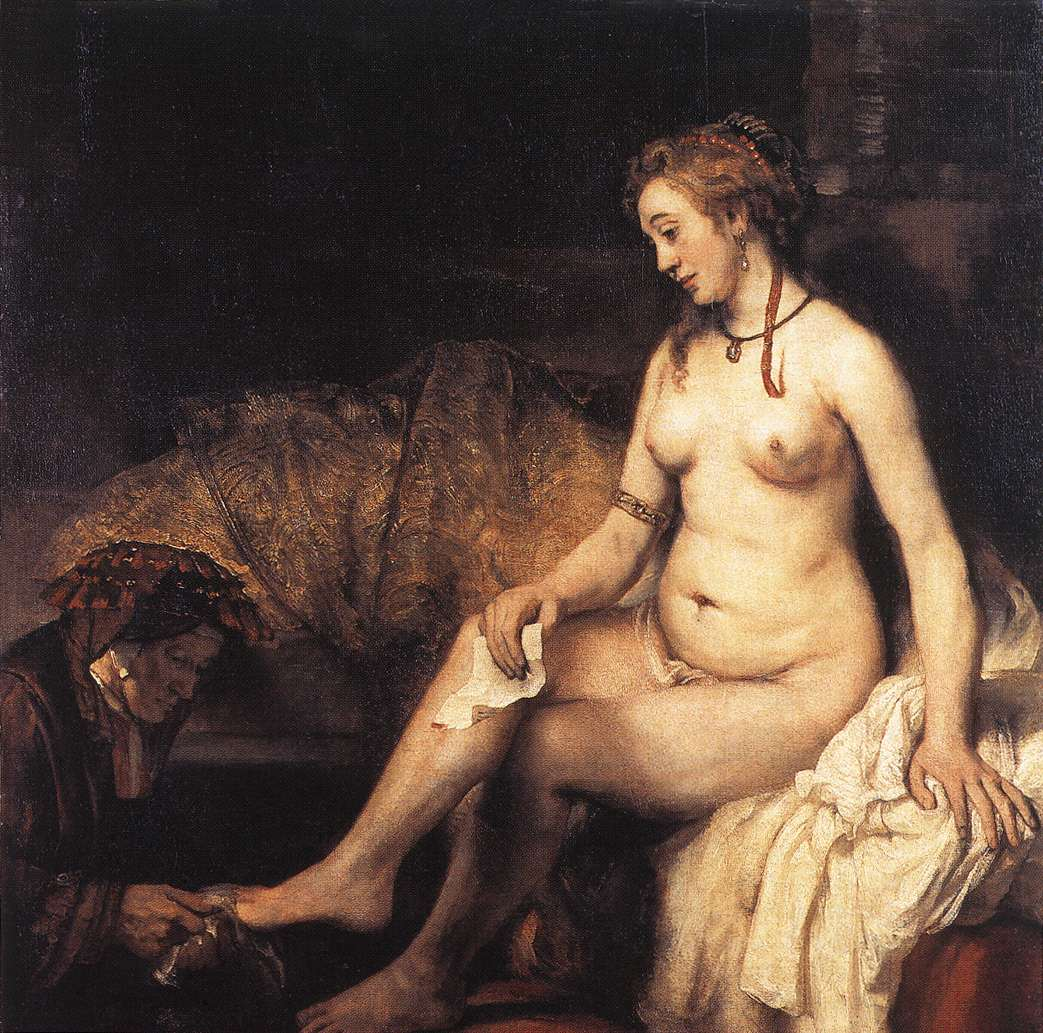
\includegraphics[height=0.15\textheight]{./img/rembrandt_bathsheba-bathing.jpg}}
	& \subfloat[\small Realismo]{\includegraphics[height=0.15\textheight]{./img/vincent-van-gogh_cart-with-red-and-white-ox.jpg}}
	& \subfloat[\small Expresionismo]{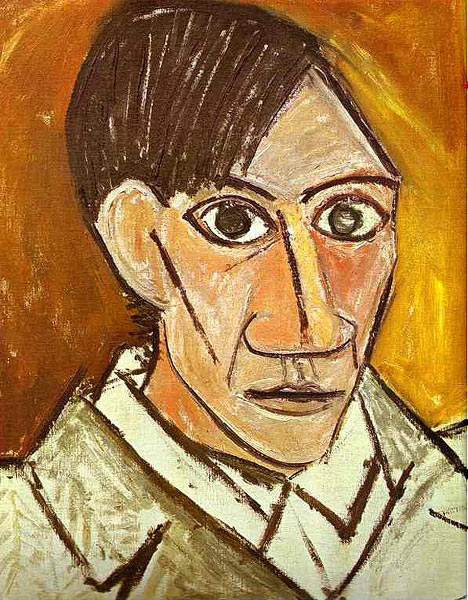
\includegraphics[height=0.15\textheight]{./img/picasso_selfport.jpg}}
      \end{tabular}

      \end{tabularx}
      \end{center}

    \end{figure}
\end{frame}

\begin{frame}
  \frametitle{Elección del número de iteraciones}
  Se detectaron 2 situaciones distintas en los resultados obtenidos:
  \begin{itemize}
    \item El estilo de la imagen resultante coincide con el estilo de la imagen propuesta.
    \item El estilo de la imagen resultante NO coincide con el estilo de la imagen propuesta.
  \end{itemize}

\end{frame}

\begin{frame}
  \frametitle{Caso 1 - Estilos coinciden}
    \begin{figure}[H]
    \captionsetup[subfigure]{labelformat=empty}
    \begin{center}
    \begin{tabularx}{\textwidth}{@{}cXX@{}}
    \begin{tabular}{cc}
      \subfloat[Imagen de Estilo: Shipwreck, Turner, 1805]{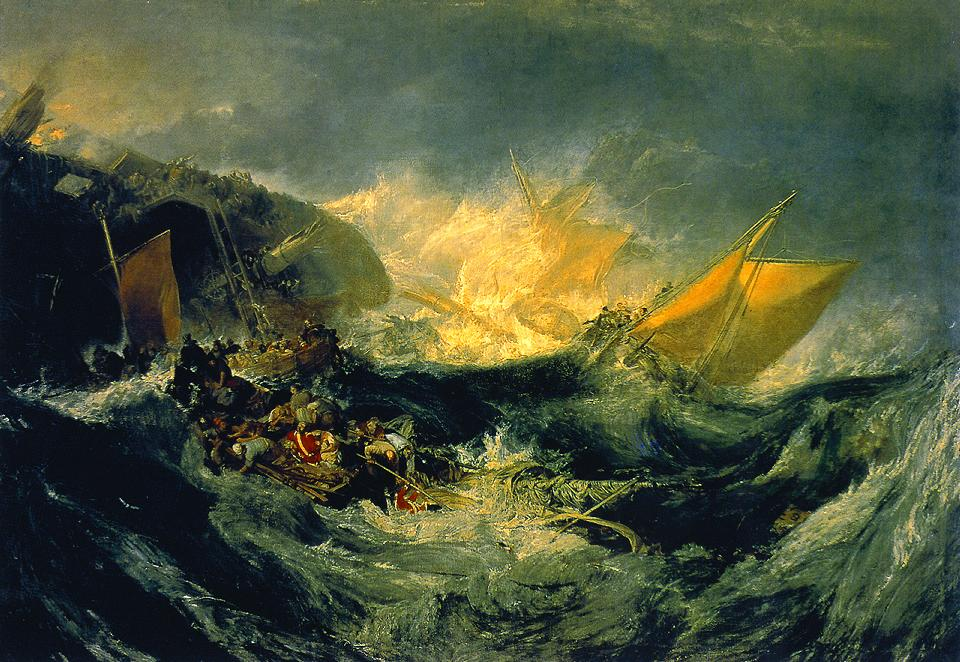
\includegraphics[height=0.3\textheight]{./img/shipwreck.jpg}}
      & \subfloat[Imagen de Contenido: Fotografía de T\"{u}bingen]{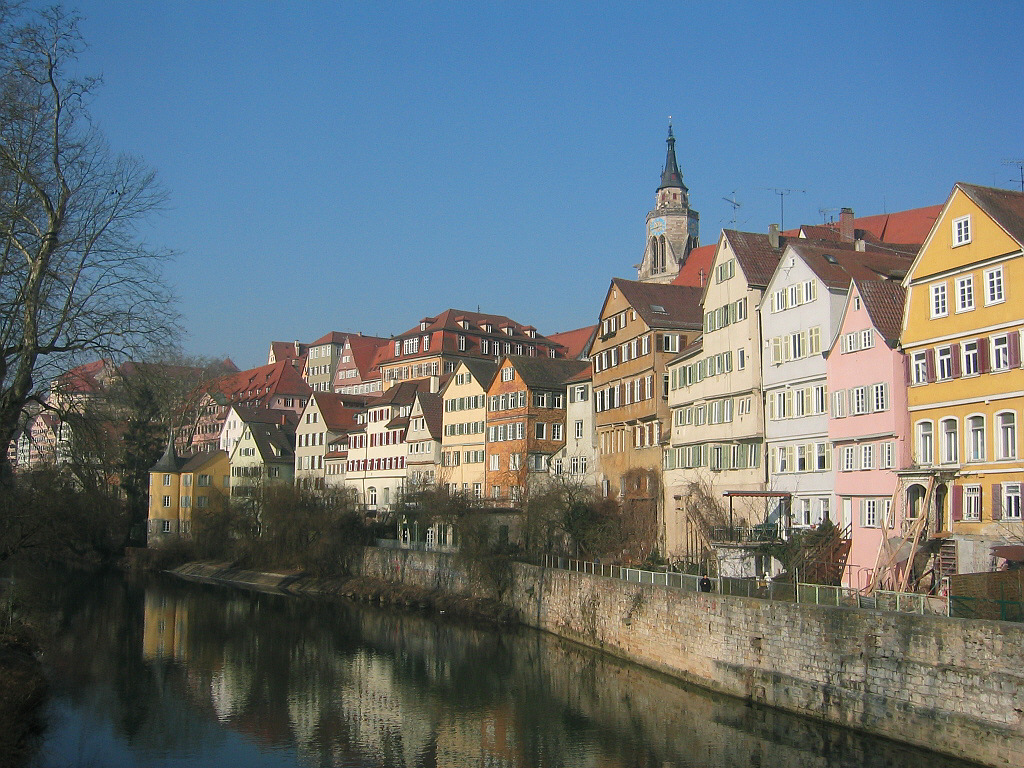
\includegraphics[height=0.3\textheight]{./img/tubingen.jpg}}\\
      \subfloat[Resultado comenzando desde ruido]{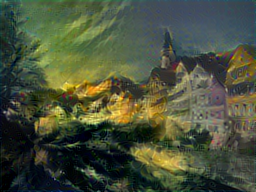
\includegraphics[ height=0.3\textheight]{./img/tubingen_shipwreck_620_random.png}}
      & \subfloat[Resultado comenzando desde el contenido]{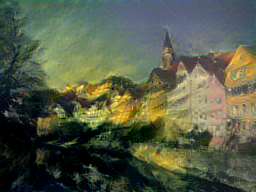
\includegraphics[height=0.3\textheight]{./img/tubingen_shipwreck_600_image.png}}\\
    \end{tabular}
    \end{tabularx}
  \end{center}
  \end{figure}
\end{frame}

\begin{frame}
  \frametitle{Caso 1 - Evolución de los puntajes}
 \begin{figure}[H]
 \captionsetup[subfigure]{labelformat=empty}
    \begin{center}
      \subfloat[Evolución de los puntajes comenzando desde ruido]{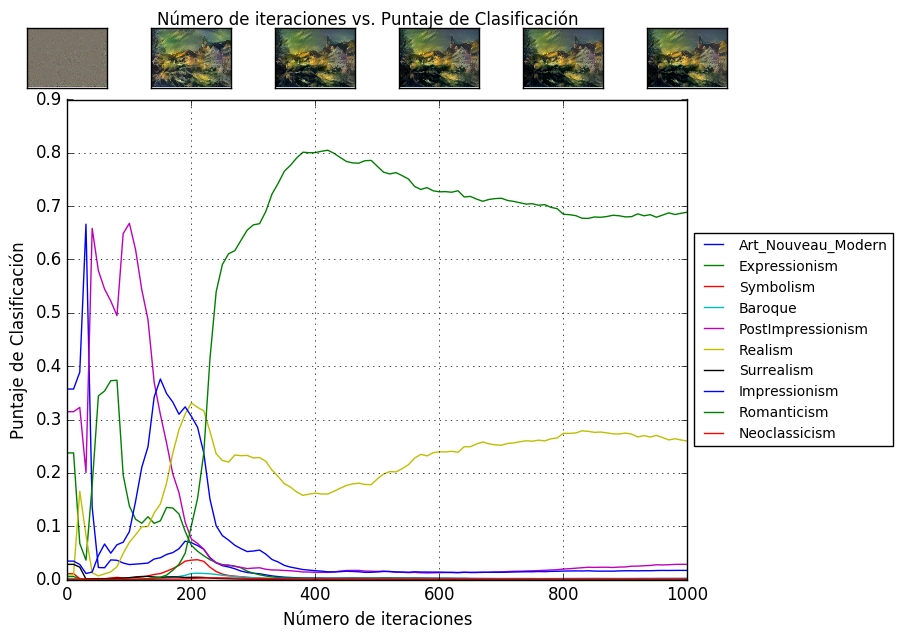
\includegraphics[ height=0.45\textheight]{./img/tubingen_shipwreck_random_scores.png}}
      \subfloat[Evolución de los puntajes comenzando desde contenido]{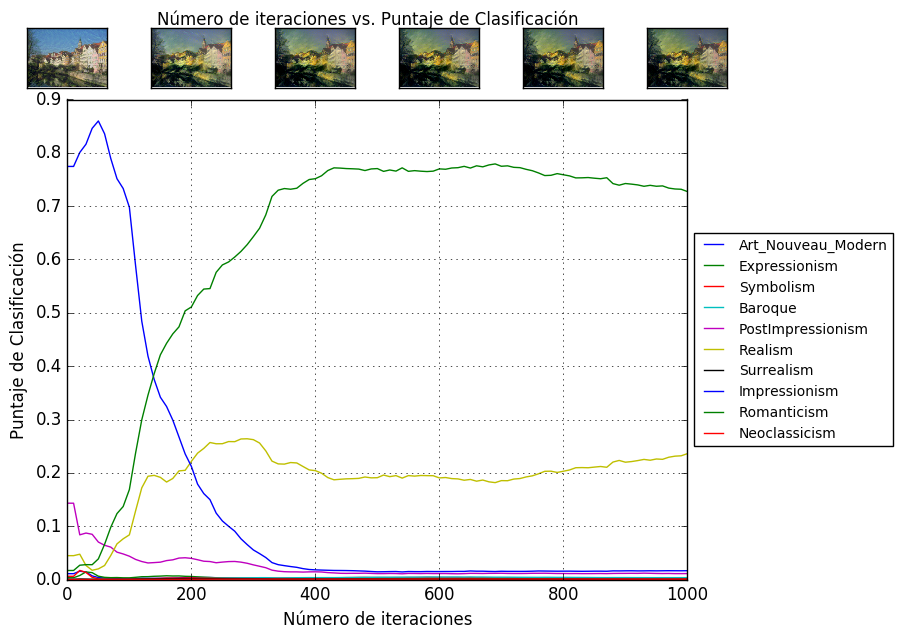
\includegraphics[height=0.45\textheight]{./img/tubingen_shipwreck_image_scores.png}}
    \end{center}
  \end{figure}
\end{frame}


\begin{frame}
  \frametitle{Caso 1 - Evolución de la calidad perceptiva}
  \begin{figure}[H]
  \captionsetup[subfigure]{labelformat=empty}
    %\def\tabularxcolumn#1{m{#1}}
    \begin{tabularx}{\textwidth}{@{}cXX@{}}
    \begin{tabular}{cc}
      \subfloat[Imagen generada en 50 iteraciones]{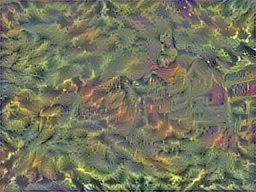
\includegraphics[height=0.3\textheight]{./img/tubingen_shipwreck_50.png}}
      & \subfloat[Imagen generada en 100 iteraciones]{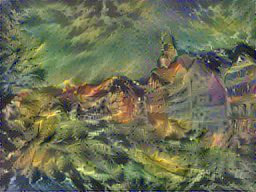
\includegraphics[height=0.3\textheight]{./img/tubingen_shipwreck_100.png}}\\
      \subfloat[Imagen generada en 200 iteraciones]{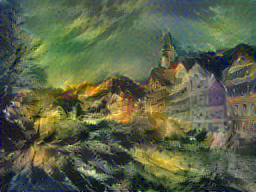
\includegraphics[ height=0.3\textheight]{./img/tubingen_shipwreck_200.png}}
      & \subfloat[Imagen generada en 600 iteraciones, elegida como óptima]{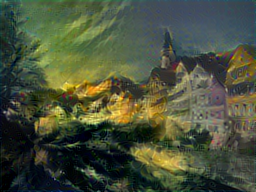
\includegraphics[height=0.3\textheight]{./img/tubingen_shipwreck_620_random.png}}\\
    \end{tabular}
    \end{tabularx}
  \end{figure}
\end{frame}

\begin{frame}
  \frametitle{Caso 2 - Estilos NO coinciden}
	\begin{figure}[H]
	\captionsetup[subfigure]{labelformat=empty}
	  %\def\tabularxcolumn#1{m{#1}}
	  \begin{tabularx}{\textwidth}{@{}cXX@{}}
	  \begin{tabular}{cc}
	    \subfloat[Imagen de Estilo: The Scream]{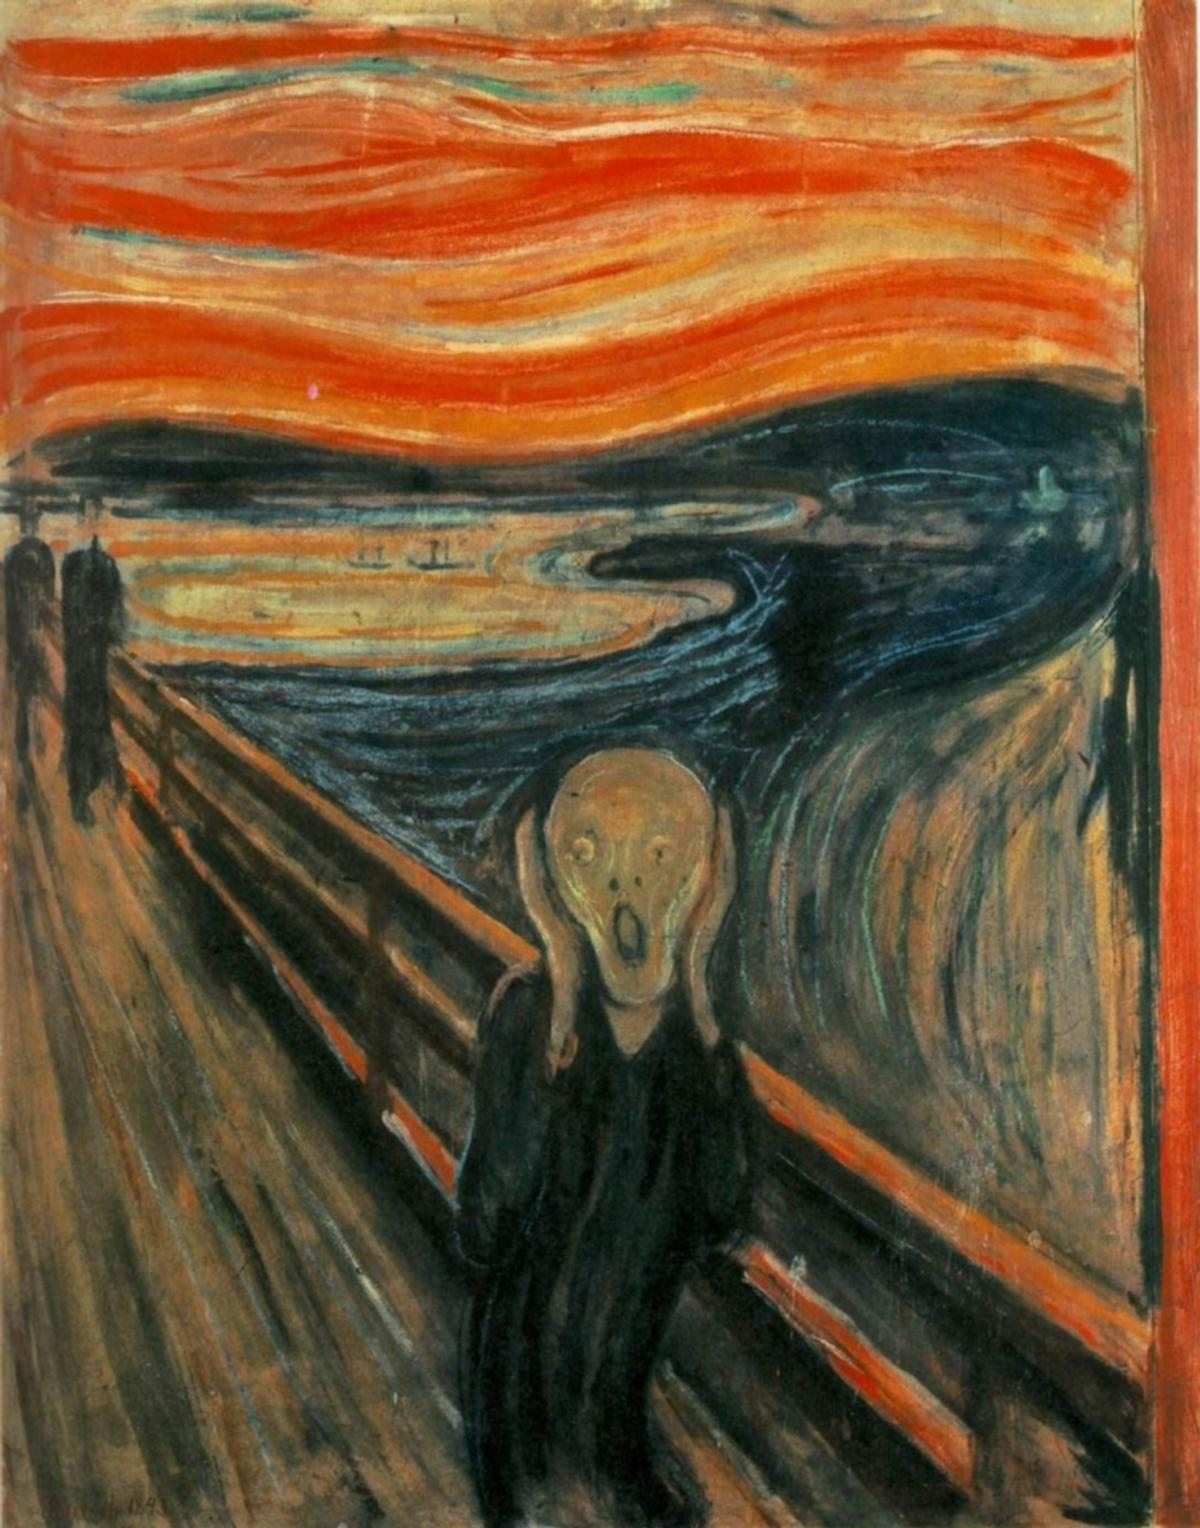
\includegraphics[height=0.3\textheight]{./img/the_scream.jpg}}
	    & \subfloat[Imagen de Contenido: Fotografía del Golden Gate]{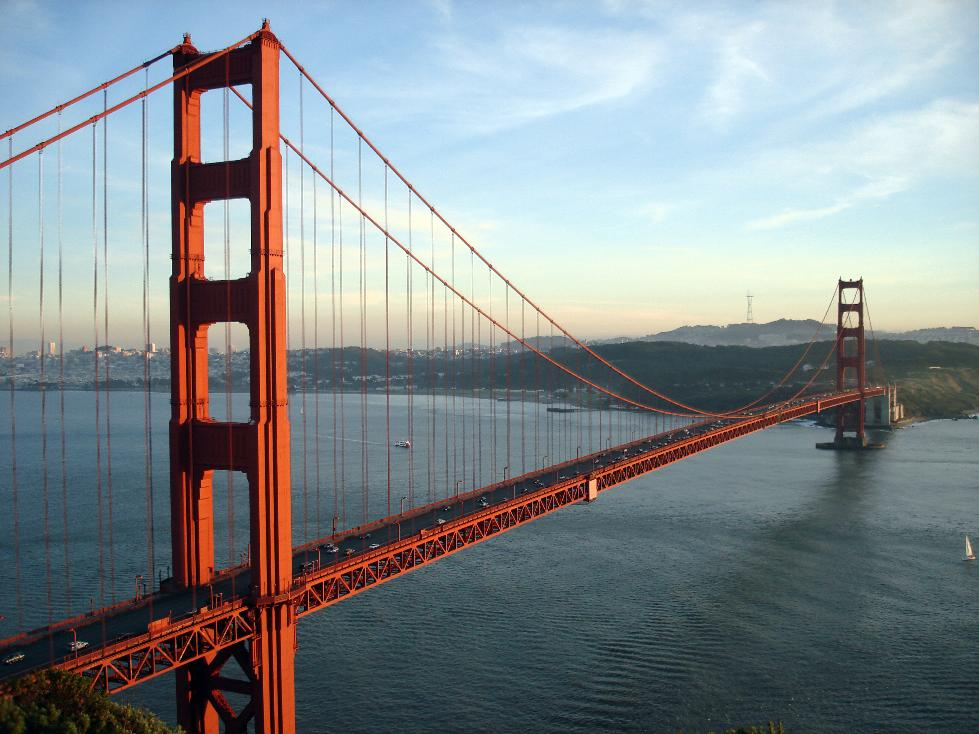
\includegraphics[height=0.3\textheight]{./img/golden_gate.jpg}}\\
	    \subfloat[Resultado comenzando desde ruido]{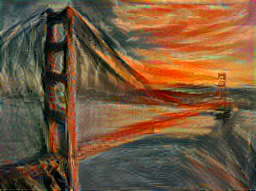
\includegraphics[ height=0.3\textheight]{./img/golden_gate_the_scream_540_random.png}}
	    & \subfloat[Resultado comenzando desde el contenido]{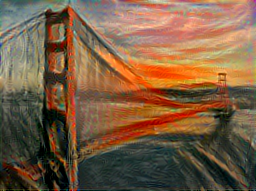
\includegraphics[height=0.3\textheight]{./img/golden_gate_the_scream_540_image.png}}\\
	  \end{tabular}
	  \end{tabularx}
	\end{figure}
\end{frame}

\begin{frame}
  \frametitle{Caso 2 - Evolución de los puntajes}
  \begin{figure}[H]
  \captionsetup[subfigure]{labelformat=empty}
    \begin{center}
      \subfloat[Evolución de los puntajes comenzando desde ruido]{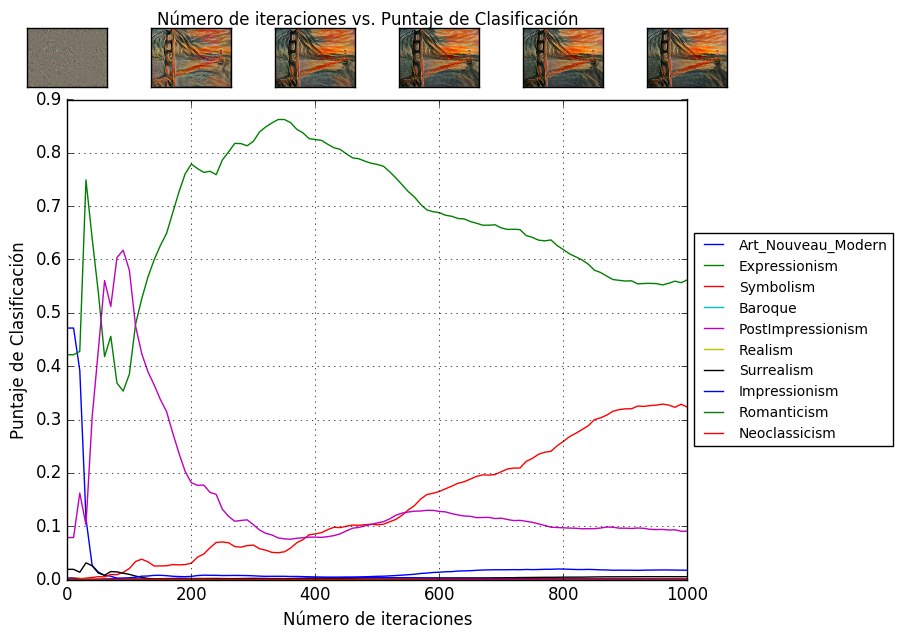
\includegraphics[height=0.45\textheight]{./img/golden_gate_thescream_random_scores.png}}
      \subfloat[Evolución de los puntajes comenzando desde contenido]{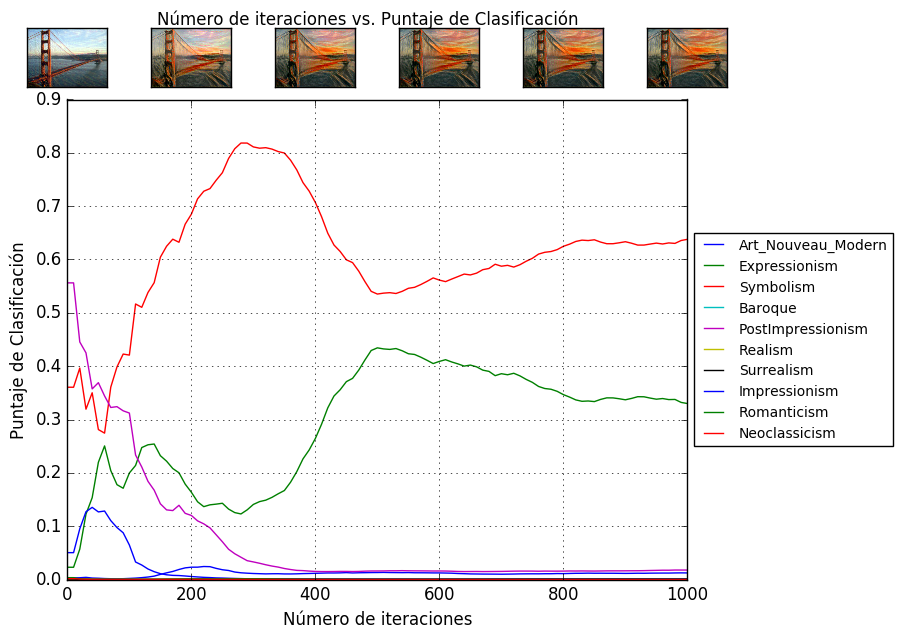
\includegraphics[height=0.45\textheight]{./img/golden_gate_thescream_image_scores.png}}
    \end{center}
    \label{fig:puntajes_caso2}
  \end{figure}
\end{frame}

\begin{frame}
  \frametitle{Caso 2 - Evolución de la calidad perceptiva}
      \begin{figure}[H]
      \captionsetup[subfigure]{labelformat=empty}
	%\def\tabularxcolumn#1{m{#1}}
	\begin{tabularx}{\textwidth}{@{}cXX@{}}
	\begin{tabular}{cc}
	  \subfloat[Imagen generada en 50 iteraciones]{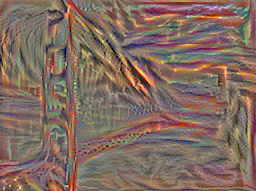
\includegraphics[height=0.3\textheight]{./img/golden_gate_the_scream_50.png}}
	  & \subfloat[Imagen generada en 100 iteraciones]{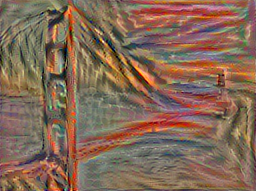
\includegraphics[height=0.3\textheight]{./img/golden_gate_the_scream_100.png}}\\
	  \subfloat[Imagen generada en 200 iteraciones]{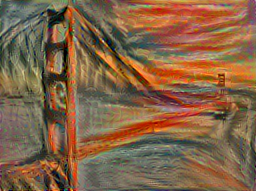
\includegraphics[ height=0.3\textheight]{./img/golden_gate_the_scream_200.png}}
	  & \subfloat[Imagen generada en 540 iteraciones, elegida como óptima]{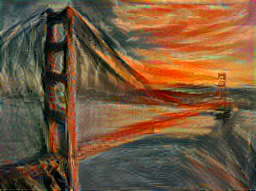
\includegraphics[height=0.3\textheight]{./img/golden_gate_the_scream_540_random.png}}\\
	\end{tabular}
	\end{tabularx}
      \end{figure} 
\end{frame}

\begin{frame}
  \frametitle{Análisis criterio de aceptación planteado}
  \begin{itemize}
    \item En base a los resultados obtenidos, se determinó que el criterio inicialmente planteado no es válido. \vspace{0.5cm}
    \item Dependiendo de la imagen de contenido y del punto de partida el estilo puede coincidir o no. \vspace{0.5cm}
    \item El criterio empírico utilizado fue determinar número de iteraciones como el punto medio del período donde alcanza un mayor puntaje de reconocimiento de estilo.
  \end{itemize}
\end{frame}

\section{Conclusiones}
\begin{frame}
  \frametitle{Conclusiones}
  \begin{itemize}
    \item El estilo de la imagen generada no depende solo de la imagen objetivo.
    \begin{itemize}
     \item Concuerda con lo que plantea Gatys et. al.
    \end{itemize}
    \vspace{0.5cm}
    \item Evaluar la imagen generada con el clasificador de estilo es un buen indicio de la calidad de la misma.
    \vspace{0.5cm}
    \item Empíricamente luego de las 300 iteraciones el resultado es aceptable y el puntaje de estilo suele entrar en una meseta.
  \end{itemize}

\end{frame}

\begin{frame}
  \vspace{1.5cm}
 {\Huge ¿Preguntas?}
\end{frame}

\end{document}
